\chapter{\label{chap:related-work}Problem description}
% Centralization of data, with the incentive of making money, naturally leads to a centralization of power. 
Music artists have a hard time making a living. The oligarchical power of music streaming services and labels squeeze the production size of the music industry. The biggest music streaming services run centralized, proprietary and closed-source software. The top 5 streaming services have a combined market share of 82\% (see \ref{tab:streaming-service-market-share}), and have huge power over both the producer and receiver sides of music streaming. Because of their power, they can ask high commission fees or lock artists to one platform. As a result, artists receive low compensation. Furthermore, the recommendation and playlist generation algorithms are a black box to the user. This gives streaming companies curatorial power. 

At the time of writing, there exists no alternative decentralized and transparent music streaming system with peer-to-peer payments directly to artists. A visualization of the economic muscle of both the label oligarchy and streaming platform oligarchy is shown in \ref{fig:current-music-publishing-situation}.

% \subsection{Ownership} ? It may be true that when you purchase a record on iTunes or favourite something on Spotify, you do not legally own a copy of it but only an access to it via their proprietary closed source platform.
\begin{figure}
    \centering
    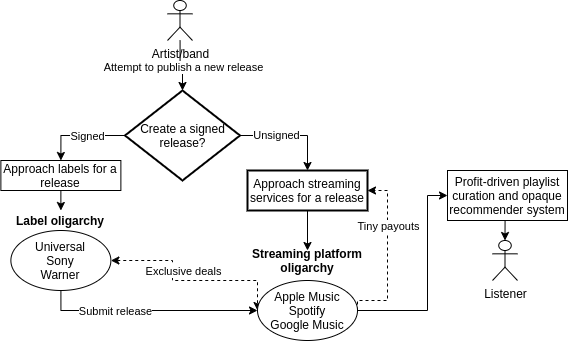
\includegraphics[width=1\linewidth]{problem-description/current-music-publishing-situation.png}
    \caption{The current flow from publishing music to receiving it as a listener. The figure shows that the framework on which music is published and found is dominated by label and streaming oligarchs and by corporate decisions.}
    \label{fig:current-music-publishing-situation}
\end{figure}

% THE REAL PROBLEMS WITH PLATFORM OLIGARCHY
% Streaming now dominates download and physical sales, accounting for 62% of US music
% revenue in 2017, a staggering 47% rise since 2012 when it accounted for only 15%
% Instead, we increasingly see label profits growing and support reserved for only
% the most successful - read marketable - artists through playlists and featured/preferred
% placement. In 2017, 93% of streams in the US went to the top 2% of available music. 
% In return for opening up their catalog of content for unlimited use, Sony, Warner and
% Universal (the Big 3) have built their contracts with streaming services to be among
% the most lucrative in the music industry. In 2011 for example, when Sony signed a
% contract allowing Spotify to use its content on their platform they were guaranteed
% over $42 million in yearly advances throughout the course of its three year lifespan,
% as well as over $9 million in ad revenue. https://www.theverge.
% com/2015/5/19/8621581/sony-music-
% spotify-contract
% It suppresses small, independent artists. 

% \todo[inline]{Mention pro-rata vs user-centric models}

% The survey findings are instead consistent with a winner-take-all or superstar model in which copyright motivates musicians through the promise of large rewards in the future in the rare event of wide popularity. This conclusion is not unfamiliar, but this article is the first to support it with empirical evidence on musicians’ revenue. 

\section{History in the industry: centralization of power}
The nature of distributing music has changed spectacularly in the last 30 years. There has been a remarkable shift from physical sales, to online track downloads and piracy issues, to digital on-demand streaming. The bargaining power in music sales was once distributed over many different physical stores and labels, but is nowadays in the hand of a few labels and Big Tech corporations. 

In the CD era of music, every city would have one or a few stores selling physical records. There were many music distribution companies competing for their sales.

With the rapid shift towards digital sales around the 2000s, IT companies used their advantage in terms of network infrastructure to sell digital copies to massive audiences. The downfall of the physical record stores began. At the same time, only a dozen digital stores managed to attract large audiences on their platforms, and thus survived. This marked the start of \textit{platform accumulation}~\citep{meier2019rising}: routing all music and money flow over centralized platforms.

Around the 2010s, the attention started to turn again to a new industry: on-demand streaming of music. In 2017, streaming accounted for 62\% of music revenue in the US, compared to only 15\% in 2012\footnote{\url{http://www.riaa.com}}. Nowadays, the number of distributors to choose from is reduced to only 5 Big Tech platforms. Together they form over 80\% share of all subscribers. Clearly, streaming royalties are an increasingly important piece of income for musicians. However, these increased revenues are not felt in the pockets of musicians, but rather in major label and platform profits.

This history shows a trend towards centralization of power in the music industry. The future of artists is in the hand of a few large corporations, as they have monopoly power over them. This comes with several issues, as explained in the next section. 

% Firstly, with only a few platforms monopolizing the market, these platforms can push down artist salaries. This mainly hits small and independent artists, as they have small bargaining power compared to major labels. Big Tech platforms have shown to make lucrative deals with major labels~\citep{meier2019rising}, paying them millions of dollars up front. Finally, they can lock content to one or a few platforms, as they have the largest music volume and audience. 

\begin{table}[]
\begin{tabular}{|l|l|}
\hline
\textbf{Streaming service} & \textbf{Market share} \\ \hline
Spotify                    & 32\%                  \\ \hline
Apple Music                & 18\%                  \\ \hline
Amazon Music               & 14\%                  \\ \hline
Tencent Music              & 11\%                  \\ \hline
YouTube Music              & 6\%                   \\ \hline
\textbf{Total}             & \textbf{82\%}         \\ \hline
\end{tabular}
\caption{Global music streaming market share, measured by subscriber share~\citep{midiamarketshare2020}}
\label{tab:streaming-service-market-share}
\end{table}

\section{Intermediaries take a large share}
Artists publishing their content on a music streaming service such as Google Music, Spotify and Apple Music receive low compensation, because the intermediaries take a large cut in revenue, typically between 25 and 40 percent (see \ref{tab:revenue-cuts}). The top 5 streaming services, controlling 80\% market share \citep{midiamarketshare2020}, have the power to ask high subscription fees. The Big Tech corporations behind these services are also tightly intertwined with dominant labels. For instance, \cite{aguiar2018platforms} notices that ``major record labels have substantial ownership stakes in Spotify''.

According to \cite{ifpi2020global}, 2019 became the first year in which digital streaming is the single biggest source of revenue for the music industry globally. At the same time, streaming services take a large cut in revenue, and artists are having a harder time making money from music. According to investigations by \cite{chris2018dissecting} and \cite{recode2015}, the revenue cut of Apple Music and Spotify is between 25\% and 30\%. An additional problem is opacity: streaming deals on these platforms remain behind closed doors. 

For these reasons, massive audiences are needed to generate sustaining profits. An investigation by Bloomberg\footnote{\url{https://www.bloomberg.com/opinion/articles/2017-09-25/the-music-business-is-more-unfair-than-ever}} shows that a whopping 152,094 Spotify subscriber streams generate \$100 on average for artists. Consequently, only 0.733\% of all acts generate enough revenue for an artist to make a living \citep{ingham2018odds}. The International Federation of the Phonographic Industry states that as of 2018 there exists a "value gap" in digital music streaming, meaning a ``mismatch between the value that some digital platforms [...] extract from music and the revenue returned to the music community–those who are creating and investing in music'' \citep{ifpi2018global}.


\begin{table}[]
\begin{tabular}{|l|l|l|l|l|l|}
\hline
\textbf{}                      & \textbf{Music release} & \textbf{Label cut} & \textbf{Platform cut} & \textbf{Artist/band cut} & \textbf{\begin{tabular}[c]{@{}l@{}}Streams per month \\ to earn min. wage \\ (solo musician)\end{tabular}} \\ \hline
TIDAL                          & Unsigned                    & 0\%                & 40\%                  & 60\%                     & 117,760                                                                                                    \\ \hline
                               & Signed                      & 55\%               & 50\%                  & 20\%                     & 353,280                                                                                                    \\ \hline
Spotify                        & Unsigned                    & 0\%                & 40\%                  & 60\%                     & 287,574                                                                                                    \\ \hline
                               & Signed                      & 55\%               & 25\%                  & 20\%                     & 862,722                                                                                                    \\ \hline
Apple Music                    & Unsigned                    & 0\%                & 40\%                  & 60\%                     & 200,272                                                                                                    \\ \hline
                               & Signed                      & 55\%               & 25\%                  & 20\%                     & 600,816                                                                                                    \\ \hline
Google Play                    & Unsigned                    & 0\%                & 40\%                  & 60\%                     & 217,752                                                                                                    \\ \hline
                               & Signed                      & 55\%               & 25\%                  & 20\%                     & 653,256                                                                                                    \\ \hline
\textbf{This thesis challenge} & Unsigned                    & 0\%                & 0\%                   & 100\%                    & \textless 75,000                                                                                           \\ \hline
\end{tabular}
\caption{Overview of revenue cuts (estimated) on streaming platforms, with a note on the streams/plays per month that an artist should have in order to make a minimum wage. The challenge of this thesis is to liberate artists from depending on intermediaries that take a large revenue cut. Sources: \cite{thetrichordist2014}, \cite{digitalmusicnews2018}.}
\label{tab:revenue-cuts}
\end{table}

\section{Platformization and gatekeeping}
The infrastructure of current internet applications are increasingly moving towards 'platformization'. In essence, platforms are taking control of ``the surface on which the market exchange take place'' \citep{andersson2016mastering} with digital distribution and network effects enabling an increasing centralization of power. This phenomenon is related to IT gatekeeping: tying access of content to a specific internet service. An example of this is the release of the album \textit{The Life of Pablo} in 2016, which was contracted to only be played on one platform, Tidal.

The latest movement in platform accumulation is the monopolization of data. Large scale of data about user interactions with the platform forms a `monopoly of knowledge' \citep{innis2007empire}. The power of platform companies are raising because platforms, in general, tend towards monopoly \citep{srnicek2017platform}. 

In relation to gatekeeping, platforms are now given the task to perform moral judgements on content, for example whether to censor a certain artist. This is controversial as these judgements are no longer in the hands of democracies but rather in the hands of companies. Recent issues exist such as the disappearance of Li Zhi\footnote{\url{https://www.independent.co.uk/news/world/asia/tiananmen-square-china-li-zhi-singer-disappears-anniversary-protests-a8940641.html}}, who published songs about democracy and social issues in China. All of China's main streaming sites removed his songs. In 2019, Apple Music also removed content from their platform by singer Jacky Cheung, who referenced the tragedies of Tiananmen Square in his songs\footnote{\url{https://hongkongfp.com/2019/04/09/apple-music-china-removes-jacky-cheung-song-reference-tiananmen-massacre/}}

\section{Slow and inaccurate royalty payments}
An additional problem of the current complex flow of intermediaries result in slow and inaccurate royalty payments. As reported by \cite{bbc2019}, Eminem's publisher sued spotify because he has never been properly paid for songs that are streamed on Spotify for billions of times. The court mentioned that the streaming service ``[...] lacked the infrastructure needed to make sure songs are licensed and musicians are paid''. Royalty payments can take 6 to 12 months to arrive at artists (TODO cite/expand). 

% In addition, these platforms use a "pro rata" model, meaning that the artists are paid per amount of plays per month. This model makes it more difficult for small, independent artists to make a living \todo{add sources}.
% Content creators on the Internet receive a low compensation for publishing their content on monopolize
% Expand upon: small independent artists. Smaller artists get low revenue, due to the "pro rata" model applied by e.g. Spotify. A user-centric model should be more fair.
\section{Monopsony power}
% \section{Centralization of power}
% Centralization of data, with the incentive of making money, naturally leads to a centralization of power
Monopsony power means that a dominant buyer has the power to push prices down with suppliers. In the context of music, this means that artists have little choice over which platform to publish their music on, because of the dominance of one platform. A few major players in the music industry together form an oligopolistic market. Monopsony power in this area can lead to squeezing the producer side. 
An example of monopsony power is an event that happened in 2014, between Amazon and Hachette. Amazon, having a large market share on e-books, used its commercial muscle to demand a larger cut of the price of Hachette books it sells. This included for all Hachette books ``preventing customers from being able to pre-order titles, reducing the discounts it offered on books and delaying shipment'' \citep{theguardian2014amazon}. 

Along the same lines, the music streaming oligarchs can use their commercial muscle to demand low pays to artists. Spotify founder and CEO Daniel Ek declared to its investors that the increase in interactions with its in-house curated playlists ``puts Spotify in control of the demand curve'' \footnote{\url{https://investors.spotify.com/financials/press-release-details/2019/Spotify-Technology-SA-Announces-Financial-Results-for-Fourth-Quarter-2018/default.aspx}}.
% \todo[inline]{move/rewrite last sentences}
% \subsection{Transparency}
% Big Tech companies obtain personal usage data to be able to improve their service, but also to to sell the data to third parties for a profit. In this process, users must heavily trust the company running the service to handle their data exactly as stated in their privacy policy. In the scope of music streaming services, user data such as browsing activity, and friends and sharing activity is obtained. For instance, Spotify saves personal usage data such as ``search queries [...], streaming history, playlists you create, your library, your browsing history, and your interactions with the Spotify Service, content, other Spotify users.'' and shares this data with advertising parties, stated in their privacy policy\footnote{\url{https://www.spotify.com/us/legal/privacy-policy}}. Google Music ``shares, processes, and maintains information about your usage, access, and playback of Your Music [...], playback activity related to items you preview and buy in the Google Music Store ("Store Usage"); and about the songs you share and listen to in connection with Google Music Social Recommendations [...]'' as described in their privacy policy\footnote{\url{https://music.google.com/about/privacy.html?em_x=22}}. 
% Following the lack of privacy comes issues with what companies do with all the user data they gather.
% Widely known is the use of user data for targeted advertising \citep{jessup2012big} and for selling as a profit \citep{yap2011user}. A risk in this process is that the third parties may use this private information for malicious purposes \citep{yap2011user}. From the perspective of the user, there is no transparency for whether this happens. According to \cite{narayanan2008robust}, privacy may be breached even when a service is willing to protect a user's privacy, because state-of-the-art de-anonymization methods do not fully make users anonymous, depending on the features stored in the database. Centralized software services are subject to a single point-of-failure. In this context this involves the risk of security breaches: if a malicious party gains access to its database, all of the records can be leaked at once which can lead to a large-scale privacy breach. Furthermore, \cite{dworkdifferential} shows that such an event can leak personal data of users who are not part of the original database.
% Integrations with IoT devices and sensors are in development which may lead to more invasion of privacy in the future.
% \subsection{Control of data}
% The GDPR contains the right for individuals to have their data erased from any platform. However, a user taking this action cannot be certain of this happening on request, as access to the companies' database is not available from the outside. Furthermore, the company implements disclosure preferences in the way they see fit, which may not be fine-grained. 
% \subsection{Content censoring}
% The company running the software is free in how and which content to censor. In addition, their content censoring policy may be changed at any time. Recent examples exist such as the disappearance of Li Zhi\footnote{\url{https://www.independent.co.uk/news/world/asia/tiananmen-square-china-li-zhi-singer-disappears-anniversary-protests-a8940641.html}}, who published songs about democracy and social issues in China. All of China's main streaming sites removed his songs. In 2019, Apple Music removed content from their platform by singer Jacky Cheung, who referenced the tragedies of Tiananmen Square in his songs.
\section{Recommendations and curatorial power}
\label{sec:problem-description-recommendations}
The Big Tech music companies recommend content that best fits their business model, which may be contrary to what is most useful to their customer. The companies can promote or dis-promote content by their choosing. This shows ``curatorial power'': the ability to advance own interests by organizing and prioritizing content \citep{prey2020locating}.

Musicians and record labels are increasingly dependent on landing on Spotify-curated playlists. For example, a study done by the European Commission shows that, for a track to land on the Spotify-curated playlist ``Today's Top Hits'', it will see an increase of \$163,000 in revenue \citep{aguiar2018platforms}. 99 of the top 100 playlists are curated by the streaming company. So its recommendation algorithms and playlist curation systems are highly influential. 

A notable problem with this situation is that the inner workings of the recommendation algorithms are opaque to the user. These algorithms, fed by user interaction data, are in some extend also a black box to the company, as they are built using machine learning technologies. However, as noted by \citep{gillespie2014relevance}, the impression that algorithms are objective is a ``carefully crafted fiction''. Namely, they are altered based on company strategies. Companies are not obliged to explain their algorithms. In the context of recommendations, this leads to a ``threat of invisibility": the problem of content regularly disappearing \citep{bucher2018if}, a phenomenon which is out of the hands of the artist, because the artist lacks knowledge in the algorithm workings. Frustrating for artists and labels is also the vagueness of getting playlisted: it is unclear why ``[...] a particular track was placed, or replaced, on a playlist'' \citep{prey2020locating}. 

On the other hand, if the `frontpage' playlists, such as ``Today's Top Hits'', are manually created by a person or company, we run into another issue. This is depicted in a recent book by \cite{heuvelings2020}. The author had the job of maintaining several high-demand playlists on Spotify, with millions of monthly listeners. This gave her substantial power but also huge pressure from artists and labels, demanding their work to be visible on her playlists. She was threatened by some of these parties as well, after which she decided to leave Spotify. This autobiography shows the immense pressure on playlist curation, when this is done by one company or person. It can make or break an artist, so there will be large (financial) pressure from labels or artists towards playlist maintainers, making the music industry unfair for smaller artists with less power.

\section{Research question}
All in all, the main issue is as follows. The music industry is imbalanced: it suffers from centralized power that is in the hand of a few labels and Big Tech corporations. Our research question thus follows:

\textit{How can we design and implement a music streaming service that distributes the power from one authority to its users?}
% \subsection{Visibility of small artists}
% Small, independent artists may suffer from major labels that invest large amounts of money to have their content promoted.
% \todo[inline]{Extend this section or merge it?}
% \subsection{Security and fault tolerance}
% As the service and software are proprietary, and the running code is closed-source, there are security risks. Specifically, the cryptography and security mechanisms used internally can not be inspected by people outside of the company. \todo[inline]{expand}
% \subsection{Server costs} ? (This is not really a problem from the perspective of user and/or artist? Unless there are sources that say otherwise)
% \subsection{Resiliency}
% At any point in time, the company running proprietary software can change, add or remove features. Its users do not necessarily have a vote in this. When a software service is sold to a different owner, the new owner can completely change direction for the service, which makes the service prone to large, possibly unwanted changes. Moreover the company can decide to take down the service in its entirety. For example: In 2017, Pandora discontinued running its service in New Zealand and Australia\footnote{\url{https://www.businessinsider.nl/pandora-shutting-down-services-australia-new-zealand-2017-7?international=true&r=US}}. In this case, users can lose all their data stored on the service.
% All the evidence suggests a description of an oligopolistic market - a few large providers with high market share, interdependence based upon pricing (chance for a kinked demand curve to be drawn, if your awarding body still uses that model!) and only slightly differentiated products.
% \subsection{Platform locking} \todo[inline]{should not be a separate section}
% As an example from YouTube, a company can disallow content creators to publish their work on other platforms, resulting creators to be locked to one platform. \todo[inline]{Find sources of this happening}  
% Related: (needs sources) https://www.bbc.com/news/technology-27694353 "But what the indies are getting really angry about is that YouTube seems to be threatening to withdraw this powerful promotional platform if they don't sign up to the new audio service - a service that will be going head-to-head with Spotify, Deezer et cetera while, as we understand it, paying considerably lower royalties."



% \subsection{Oligopoly formation}
% Also, a natural consequence: (Unnecessary high) pricing of content. When a monopoly on music content is formed, the Big Tech companies can together decide to up the price 'whenever they feel like it'.
% \subsection{Copyright orthodoxy} ?
% % https://search.proquest.com/openview/2ea25b1bed66750c91cdbc6ea2a5093a/1
% \subsection{Low level of innovation} ?

% \todo[inline]{Software quality measurements: functionality, scalability, maintainability, portability, and, ingeneral, enhancing the usability of the software. See \citep{raghunathan2005open}}

% From Audius Whitepapter:
% We see a number of specific challenges faced by creatorsand listeners today:1.  There is little to no transparency around the originsof creator payouts (e.g.  number of plays, location,original gross payment before fees)2.  Incomplete  rights  ownership  data  often  preventscontent  creators  from  getting  paid;  instead,  earn-ings accumulate in digital service providers (DSPs)and rights societies3.  There are layers of middlemen and significant timedelay involved in payments to creators4.  Publishing rights are complicated and opaque, withno incentives for the industry to make rights datapublic and accurate5.  Remixes,  covers,  and  other  derivative  content  arelargely censored due to rights management issues6.  Licensing issues prevent DSPs and content from be-ing accessible worldwide


% Spotify’s front page “Browse” screen presents a classic illusion of choice, a stream of genre and mood playlists, charts, new releases, and now podcasts and video. It all appears limitless, a function of the platform’s infinite supply, but in reality it is tightly controlled by Spotify’s staff and dictated by the interests of major labels, brands, and other cash-rich businesses who have gamed the system. https://thebaffler.com/salvos/the-problem-with-muzak-pelly
% “The more vanilla the release, the better it works for Spotify. If it’s challenging music? Nah,” 
% We should call this what it is: the automation of selling out.
% “The difference now is that, if you don’t bow down to Spotify, you might as well tell whoever runs the guillotine that’s above your neck to just let her rip,” Saunier says, as the band sits in their van, on tour, en route from Grand Rapids to Detroit. “These streaming services are literally the only option for a music career nowadays.”

% https://www.volkskrant.nl/mensen/bij-spotify-kon-dieuwertje-heuvelings-artiesten-maken-of-breken-ze-schreef-er-een-roman-over~b274536aa/

% Just two days after Frank Ocean’s “Blonde”—one of the biggest releases of theyear—released on Apple’s iTunes, Lucian Grainge, CEO of Universal Music Group(UMG)—and widely regarded as the most powerful executive in the musicindustry—reportedly ordered the company’s labels to stop the practice of making“exclusive” distribution deals with streaming services. One day later, the tracks wereordered to be shut down from Spotify and Apple music by UMG against Frank’s wishes.These centralized services had to comply. Frank Ocean could be facing charges of up to$2 million USD against UMG and other recording outlet